\chapter{Reconocimiento Automático de Matrículas}
Figura X. Ejemplo de Sistema Inteligente de Transporte con Cámaras de Seguridad \cite{TechFAQ2016-oi}

El reconocimiento automático de matrículas (en inglés, Automatic License Plate Recognition o ALPR) es uno de los módulos (importantes de los Sistemas Inteligentes de Transporte (ITS). Investigaciones de \cite{Anagnostopoulos2008-uh} y \cite{TechTarget2016-gw} mencionan múltiples aplicaciones de ALPR, tales como la determinación de qué vehículos pertenecen o no en un parqueo, disposición de pases parqueo eliminando la necesidad de confirmación humana, recuperación de autos robados, control de tráfico, etc..

Usualmente, un módulo de ALPR se divide en tres etapas principales: detección de la matrícula de una imagen o video, segmentación de caracteres y, reconocimiento de caracteres. Entre estos, la detección de la matrícula es la parte más importante y la más difícil; los módulos ALPR deben enfrentar factores no problemáticos como: imágenes fuera de foco, condiciones de iluminación no deseadas, matriculas pequeñas, sombras y diferentes condiciones climáticas \cite{Mahini2006-us}.
A pesar de que se han realizado muchas investigaciones en el área del ALPR, los sistemas actuales tienen un buen desempeño bajo condiciones específicas \cite{Anagnostopoulos2006-is}, tales como: distancia de la cámara \cite{Martin2002-zu,Guo2008-qk}, velocidad del vehículo \cite{Garibotto2001-lu}, condiciones de iluminación \cite{Xiong2004-qv,Mahini2006-us}, posiciones de la cámara \cite{Chang2004-kg}, etc. No olvidemos que los módulos ALPR pueden fallar en el borde de dos países debido a las variaciones en los patrones patrones de los caracteres en matrículas \cite{Anagnostopoulos2006-is,Shapiro2006-rv,Mecocci2006-nt}.

  \begin{figure}[H]
        \centering
        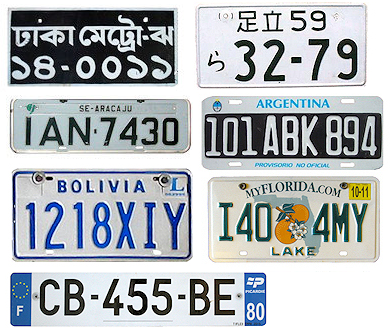
\includegraphics[width=0.80\textwidth]{worldcarplates}
        \caption{ Matrículas de diferentes países \protect\cite{Kustermann2016-yd}}
        \label{fig:worldcarplates}
\end{figure}  

La figura \ref{fig:worldcarplates} muestra claramente cómo las matrículas de un país a otro varían bastante. Por esta razón no es efectivo utilizar un módulo ALPR desarrollado para un país, en otro, sin antes haberlo adaptado.
\section{Detección vs. Reconocimiento}
La\textit{ detección} de objetos consiste en determinar si en una imagen o video arbitrarios hay un objeto determinado (un rostro, un auto) y, en caso haberlo, en qué posición se encuentra. Por otro lado, el \textit{reconocimiento }de objetos (el rostro de Juan, el auto de Pedro) consiste en comparar el objeto detectado contra una base de datos para saber si existe alguna asociación con alguno registrado. Vale mencionar que es usualmente más difícil la detección de objetos en la escena compleja de una imagen que el reconocimiento de los mismos. Dado lo anterior, la mayoría de los algoritmos de reconocimiento pueden ser usados para la detección de objetos. Sin embargo, dependiendo del objeto a detectar, unos métodos pueden ser más adecuados que otros \cite{Ekvall2005-ut}.
\section{OpenALPR}
OpenALPR es una librería open-source de visión artificial que se encarga de la tarea del reconocimiento automático de matrículas utilizando los módulos de OpenCV para realizar el procesamiento de imágenes..
  
  \begin{figure}[H]
        \centering
        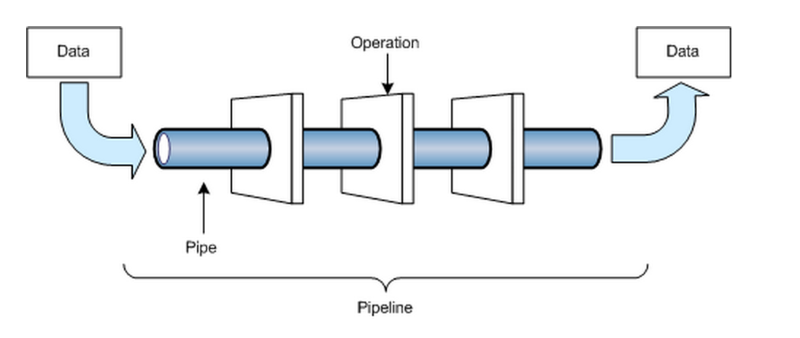
\includegraphics[width=0.90\textwidth]{openalpr-pipeline}
        \caption{Representación gráfica de una cadena de procesos (en ingles, Pipeline) \protect\cite{Saini2015-yp}}
        \label{fig:openalpr-pipeline}
\end{figure}
    
A continuación se describe cada uno de los subprocesos que realiza la librería OpenALPR para el reconocimiento de una matrícula a partir de una entrada, sea una imagen o un video. 

\subsection{OpenCV}
OpenCV es una librería open-source bajo la licencia BSD que contiene cientos de algoritmos de visión artificial, utilizada por Google, Microsoft, IBM, Intel, etc. \cite{OpenCV2016-bv}. OpenCV tiene una estructura modular distribuida de la siguiente manera:
\begin{itemize}
\item \textbf{core} - define las estructuras de datos y las funciones básicas utilizadas por todos los otros módulos.
\item \textbf{imgproc} - módulo de procesamiento de imágenes que incluye filtros lineales y no lineales, transformaciones geométricas (resize, affine y perspective warping, generic table-based remapping), inversión del espacio de colores, histogramas, etc.
\item \textbf{video} - módulo de análisis de video que incluye estimación de movimiento, sustracción de fondo y algoritmos de seguimiento de objetos.
\item \textbf{calib3d} - módulo de algoritmos básicos de multiple-view geometry, calibración singular y estéreo de cámaras, estimación de pose de objeto, algoritmos de correspondencia estéreo y, reconstrucción de elementos 3D.
\item \textbf{features2d} - módulo de detectores de características sobresalientes, descriptores y, igualadores de descriptores.
\item \textbf{objdetect} - módulo de detección de objetos e instancias de clases predefinidas (por ejemplo, rostros, ojos, tazas, personas, autos, etc.)
\item \textbf{highgui} - módulo con una interfaz intuitiva para la captura de video, codecs de imágenes y video y capacidades de UI sencillas
\item \textbf{gpu} - módulo con algoritmos acelerados para el GPU de diferentes módulos de OpenCV
\item ... y otros módulos de ayuda como FLANN y envoltorios de pruebas de Google, bindings para Python, etc.    
\end{itemize}


\section{Pre-Procesamiento}
El pre-procesamiento puede ser útil para acelerar el proceso de cómputo a la hora de detectar un objeto. Por ejemplo, si se quiere realizar un reconocimiento de rostros en tiempo real a través de una transmisión de video en alta calidad, la computadora debe manejar grandes cantidades de pixeles por segundo y, presentarlos a un algoritmo de reconocimiento de patrones puede ser computacionalmente factible. 

El objetivo del pre-procesamiento es encontrar características que se obtengan rápidamente y que mantengan información útil para la discriminación de clases. Por ejemplo, el valor medio de la intensidad en una subregión rectangular en una imagen puede ser calculado de una manera muy eficiente \cite{Viola2004-bx}, y un conjunto de estos descriptores puede ser muy efectiva para la rapida deteccion de rostros.

No obstante, se debe tener cuidado con los métodos de preprocesamiento porque frecuentemente se descarta información; y, cuando esta información es importante para las solución del problema entonces la precisión total del sistema puede fallar \cite{Bishop2007-am}.

\section{Detección de Matrículas}
La fase de detección sucede una vez por cada imagen recibida (entrada). OpenALPR utiliza el algoritmo LBP (usualmente utilizado para la detección de rostros) para encontrar regiones posibles que contengan matrículas (x, y, ancho, alto). Luego, cada una de estas regiones se envía a los siguientes subprocesos de la cadena.

La fase de detección es usualmente la de mayor intensidad computacional; para solventar esto se la puede acelerar por GPU para mejorar el desempeño. 

\subsection{Medida de Error de un Detector}

\subsection{Algoritmo del Patrón Binario Local}
El reconocimiento de objetos mediante visión artificial involucra dos aspectos importantes \cite{Huang2011-ud}: representación del objeto \cite{Ahonen2006-gg} y diseño del clasificador \cite{Cover1967-vb,Wright2009-en,Cortes1995-qx}. La representación del objeto consiste en obtener un conjunto de características relevantes que describan el objeto, a partir de las imágenes originales. Las características “buenas” deben \cite{Hadid2004-dk}:

\begin{itemize}
\item Tolerar cierta variación pero igualmente discriminar estrictamente otras clases
\item Ser de fácil extracción a partir de una imagen en formato original para permitir el rápido procesamiento
\item Existir en un espacio de baja dimensionalidad para evitar el uso de clasificadores costosos
\end{itemize}

En el momento de su creación, el algoritmo LBP tuvo el propósito de ser utilizado para la describir texturas y en representación de rostros \cite{Ahonen2006-gg}; vale mencionar que a lo largo de los años se ha observado un mayor interés en su uso para la representación facial.

El operador LBP, introducido por \cite{Ojala1996-el}, codifica los pixeles de una imagen comparándolo con sus ocho pixeles vecinos en un área de 3x3 partiendo de la esquina superior izquierda. Los valores menores son codificados con 0 y los otros con 1. Los números se concatenan en sentido del reloj partiendo de la esquina superior izquierda para generar un número binario, del cual se obtiene el equivalente en decimal. Este número decimal es conocido como el código LBP. 

A partir de una imagen, o región de una imagen, se puede obtener un histograma de los códigos LBP observados en los pixeles de la región. Este histograma es también llamado un descriptor LBP o patrón LBP.
Posteriormente, \cite{Ojala2002-pl} propusieron dos extensiones al operador original. Primero, el operador fue extendido para poder cambiar el radio de la vecindad y la cantidad de vecinos y así poder capturar características dominantes en diferentes escalas. Segundo, propusieron utilizar un subconjunto de los $2^P$ patrones generados por LBP en una región para describir la textura de las imágenes. Estos patrones, llamados patrones uniformes, contenían como máximo dos transiciones de 0 a 1 en su cadena de bits, donde 00111000 tiene dos transiciones y 00010011 no. La idea de utilizar únicamente estos patrones uniformes es debido a que en ellos se encuentra la mayor parte de la información de las texturas en una imagen. 

\subsection{Descriptores LBP}
La imagen de un objeto puede considerarse como una composición de los micro-patrones LPB. Al generar un histograma LBP a partir de la imagen, se obtiene las ocurrencias de los micro-patrones pero no su ubicación en la imagen. 

Ante esto, \cite{Ahonen2006-gg} propuso, de la siguiente manera:
\begin{enumerate}
    \item dividir las imágenes de rostros en M subregiones “relevantes” para la extracción de múltiples histogramas LBP locales y luego, 
    \item concatenar estos descriptores en un histograma global resultante con la información espacial de cada uno.

\end{enumerate}

El histograma resultante propuesto describe tanto información sobre la textura local como la forma global del objeto.
No obstante, al ser la selección de subregiones relevantes arbitraria, se adoptó AdaBoost, con lo que se obtuvo una cascada de clasificadores impulsados (cascade of boosted classifiers). Adaboost \cite{Viola2001-rh} ayuda seleccionando las subregiones más discriminativas, a partir de un conjunto de subregiones generadas al rotar y escalar una sub-ventana sobre la imagen del objeto. 

\subsection{Entrenamiento de un detector}
Primeramente, un clasificador (específicamente, una cascada de clasificadores impulsados, utilizando con características LBP) es entrenado con unos cientos de imágenes ejemplo de un objeto particular (por ejemplo, un rostro o un auto); estos son llamados ejemplos positivos y deben ser del mismo tamaño (por ejemplo, 20x20). De igual manera, se deben proporcionar ejemplos negativos - imágenes arbitrarias del mismo tamaño que no contengan al objeto.

Después de que el clasificador es entrenado, puede ser aplicado a una región de interés en una imagen de entrada. El clasificador genera una salida de 1 si en la región es probable que exista el objeto (rostro, auto) y 0 en caso contrario. Para buscar el objeto en la imagen se puede mover y ajustar el tamaño de la ventana a lo largo de la imagen y verificar si existe el objeto utilizando el clasificador. Entonces, para encontrar un objeto de un tamaño desconocido en una imagen el proceso de escaneo debe ser realizado múltiples veces y en diferentes escalas \cite{OpenCV2016-vq}


\subsection{Cascada de Clasificadores Impulsados}
Para determinar si en una imagen se encuentra una objeto o no, el algoritmo divide la imagen integral en subregiones de tamaños diferentes. Cada subregión es procesada por una serie de clasificadores donde cada uno evalúa si la subregión es el objeto buscado o no.

La palabra “cascada” en el clasificador significa que el clasificador resultante está compuesto por múltiples clasificadores más simples que trabajan en cadena (cascada) sobre una región de interés hasta que una región candidata es rechazada o todos los clasificadores generan resultados positivos. La palabra “impulsado” (boosted) significa que los clasificadores en cada etapa de la cascada son por sí mismos complejos y están compuestos por clasificadores básicos, utilizando un métodos de boosting. El más conocido históricamente es Adaboost. Los clasificadores básicos son clasificadores por árbol de decisión compuestos de por lo menos dos hojas.

La utilización de este algoritmo supone un ahorro de tiempo considerable ya que no serán procesadas subregiones de la imagen que no se sepa con certeza que contienen al objeto y sólo se invertirá tiempo en aquellas subregiones que posiblemente si lo contengan. \cite{Viola2001-rh}

\section{Binarización}
Como fue descrito en el Cap. Procesamiento de Imagenes Digitales bajo la seccion de Segmentacion de Imagenes Digitales, para la binarización de la imagen se elige un umbral de intensidad y se asigna los valores de los pixeles para distinguir regiones en la imagen.

Esta fase y todas las subsiguientes, ocurren múltiples veces (una por cada región que posiblemente contenga una matrícula)

En este caso, se generan múltiples imágenes binarias para no perder información sobre los caracteres en la imagen. La binarización utiliza el método Wolf-Jolion y el método Sauovola con varios parámetros \cite{Wolf2004-so,Oliveira2009-io}. Cada una de las imágenes binarias son procesadas en las fases subsiguientes.
\section{Análisis de Caracteres}
El análisis de caracteres intenta encontrar regiones de tamanhos de caracteres en la región de la matrícula. Primero encuentra todas las masas amorfas (blobs) en la región de la matrícula. Luego, busca las masas amorfas que son aproximadamente del tamaño y ancho de un carácter de una matrícula y tienen “bases y alturas” que están en una línea recta con las otras masas amorfas que tengan un ancho/alto similar.

Este análisis se hace múltiples veces en la región; comienza primero con caracteres pequeños y luego busca caracteres más grandes.

Si no se encuentra nada en la región, esta es descartada. No obstante, si se encuentra potenciales caracteres, la región se guarda y se procesa más a fondo.
\section{Detección de Bordes}
La siguiente fase es encontrar los bordes de la matrícula. Vale mencionar que la fase detección sólo es responsable por identificar regiones posibles donde exista una matrícula. Frecuentemente provee una región que es un poco más grande o más pequeña que la matrícula real. La detección de bordes trata de encontrar con precisión los bordes superior/inferior/izquierdo/derecho de la matrícula.

Para encontrar todas las líneas verticales y horizontales, se utiliza la transformada de Hough \cite{OpenCV2016-kr}.

Se utiliza esta lista de líneas y la altura de los caracteres (computada en Análisis de Caracteres) para encontrar los bordes de la matrícula más probables. Utiliza pesos configurables para determinar qué borde tiene más sentido de ser un borde de la matrícula. Intenta utilizar un borde por defecto (en base al ancho/alto ideal de la matrícula) para ver si es una buena pareja.

\section{Enderezamiento}
Dados los bordes de la matrícula, la fase de Enderezamiento reorganiza la región de la placa a un tamaño y orientación estándar. Idealmente, esto devuelve una matrícula orientada correctamente (sin rotación o propio enderezamiento).

\section{Enderezamiento}
La segmentación de caracteres intenta aislar todos los caracteres contenidos en la imagen de la matrícula. Utiliza un histograma vertical para encontrar los espacios entre los caracteres de la matrícula. Esta fase también limpia el caracteres removiendo las masas amorfas pequeñas y desconectadas y descalificando regiones de caracteres que no son lo suficientemente altos. De igual manera, intenta remover regiones “borde” para que el borde de la matrícula no sea clasificado equivocadamente como un número “1” o una letra “l”. 

\section{Reconocimiento Óptico de Caracteres (OCR)}
El reconocimiento óptico de caracteres permite reconocer caracteres en texto escrito \cite{Mithe2013-yn}. La fase de OCR analiza cada carácter independientemente: para cada imagen segmentada, computa todos los caracteres posibles  y sus grados de confianza a través de Tesseract \cite{Tesseract-OCR2016-fe}.
\section{Post-Procesamiento}
Dada una lista de todos los posibles caracteres OCR y sus confianzas, el post-procesamiento determina las mejores combinaciones de letras para la matrícula, organizadas en una lista de top N. El post-procesamiento descarta todos los caracteres por debajo de un umbral específico. 

De igual manera, el post-procesamiento maneja la validación de región si esta opción está habilitada. Por ejemplo, se puede especificar la región “Missouri” y el post-procesamiento intenta emparejar los resultados con una plantilla del formato de las matrículas de Missouri. Dada una plantilla de tipo  [char][char][number]-[char][num][char] y la lista de matrículas más probables:
\begin{itemize}
    \item CFOCIG
    \item CF0CIG
    \item CF0C1G

\end{itemize}

La tercera entrada concuerda con la plantilla, y las dos primeras no; entonces, post-procesamiento indicará que la tercera entrada es la mejor opción.

